\documentclass[a4paper,12pt]{article}

\usepackage[utf8]{inputenc}
\usepackage[T1]{fontenc}
\usepackage[brazil]{babel}
\usepackage{amsmath, amssymb}
\usepackage{graphicx}
\usepackage{geometry}
\usepackage{booktabs}
\usepackage{xcolor}
\usepackage{float}
\usepackage{hyperref}
\usepackage{setspace}

\geometry{top=3cm, bottom=2.5cm, left=3cm, right=2cm}
\onehalfspacing

\title{\textbf{Estudo de Viabilidade Econômico-Financeira:\\Marketplace B2B para o Setor de Construção Civil}}
\author{Relatório de Análise de Risco Operacional e Institucional}
\date{\today}

\begin{document}

\maketitle
\begin{abstract}
Este relatório apresenta a modelagem econômico-financeira de um marketplace B2B voltado ao setor de construção civil, utilizando diretrizes institucionais de *Venture Capital*. Com o intuito de neutralizar o viés otimista comum a projetos *early-stage* (fenômeno conhecido como \textit{Garbage In, Garbage Out}), o modelo adota premissas conservadoras: elevada taxa de desconto devido ao risco de mortalidade (\textit{WACC} em níveis de *Seed Stage*), mitigação drástica nas taxas de conversão de clientes e contabilização de fricções operacionais, como custos com \textit{gateways} de pagamento e o risco inerente de *bypass* (fuga de transação) por parte das construtoras. As análises englobam o dimensionamento de *Unit Economics*, Otimização Linear e Simulação de Cenários Estocásticos (Monte Carlo) para testar a resiliência da tese.
\end{abstract}

\tableofcontents
\newpage

\section{Introdução e Premissas de Risco}

Plataformas de intermediação B2B em setores analógicos (como a construção civil) enfrentam longos ciclos de venda, desconfiança institucional e forte incentivo econômico para desintermediação de transações (*bypass*). 

Este relatório não tem a intenção de superestimar a adoção da plataforma. Pelo contrário, as premissas deste estudo de viabilidade foram parametrizadas sob a ótica de estresse e risco máximo:
\begin{enumerate}
    \item \textbf{Custo de Aquisição e Baixa Conversão:} Diferente de ferramentas SaaS de baixo atrito, assumiu-se que os canais de captação (Google Ads, Outbound) terão uma taxa de conversão final de apenas \textbf{5\%}, forçando os limites do CAC para a faixa de R\$ 4.500 a R\$ 15.000 por construtora.
    \item \textbf{Risco de \textit{Bypass}:} Assumiu-se que a plataforma não conseguirá capturar o GMV integral da obra. Devido a negociações diretas entre fornecedores e construtoras por fora do sistema, estima-se que a captura transacional seja de apenas \textbf{50\%} do custo de materiais.
    \item \textbf{Custos Adquirentes (COGS):} Para sustentar uma taxa transacional (*take rate*) de 2,5\%, a operação incorre em pesados custos de \textit{gateway} ou *split* de pagamento (estimados em 1\% sobre o GMV capturado), corroendo severamente a Margem Bruta no momento da liquidação.
\end{enumerate}

\section{Dimensão de Mercado (TAM, SAM, SOM)}

O dimensionamento atua sob bases macroeconômicas \cite{ibge2025}:
\begin{itemize}
    \item \textbf{TAM (Total Addressable Market):} Estimado em R\$ 64,12 Bilhões, baseado em 50.000 obras/ano no Brasil.
    \item \textbf{SAM (Serviceable Available Market):} R\$ 12,82 Bilhões (20\% do TAM focado no mercado formalizado).
    \item \textbf{SOM (Serviceable Obtainable Market):} Meta de captura conservadora para o Ano 5 atingindo cerca de 1.264 obras.
\end{itemize}

\section{Unit Economics e Otimização Linear}
\subsection{CAC, LTV e Custo de Transação}
Com a conversão reduzida a 5% e o *bypass* de 50%, a Receita Líquida projetada por obra despenca para cerca de R\$ 16.031. No entanto, o \textit{Life Time Value} (LTV) ainda se mantém estável na ordem de \textbf{R\$ 120.234,00} ao longo do ciclo de vida do cliente de 5 anos.

O Custo de Aquisição (CAC) subiu de forma acentuada, no entanto, o modelo relata que a relação LTV/CAC gira em torno de \textbf{14,3x} a \textbf{61,2x}. Na realidade do *Venture Capital*, múltiplos acima de 4x já justificam o crescimento. A justificativa para esse índice alto é a natureza volumosa do ticket médio transacionado na construção civil; ainda que se gaste R\$ 15 mil para adquirir o cliente, o *fee* sobre uma única obra (mesmo com *bypass*) paga rapidamente a aquisição.

\begin{figure}[H]
    \centering
    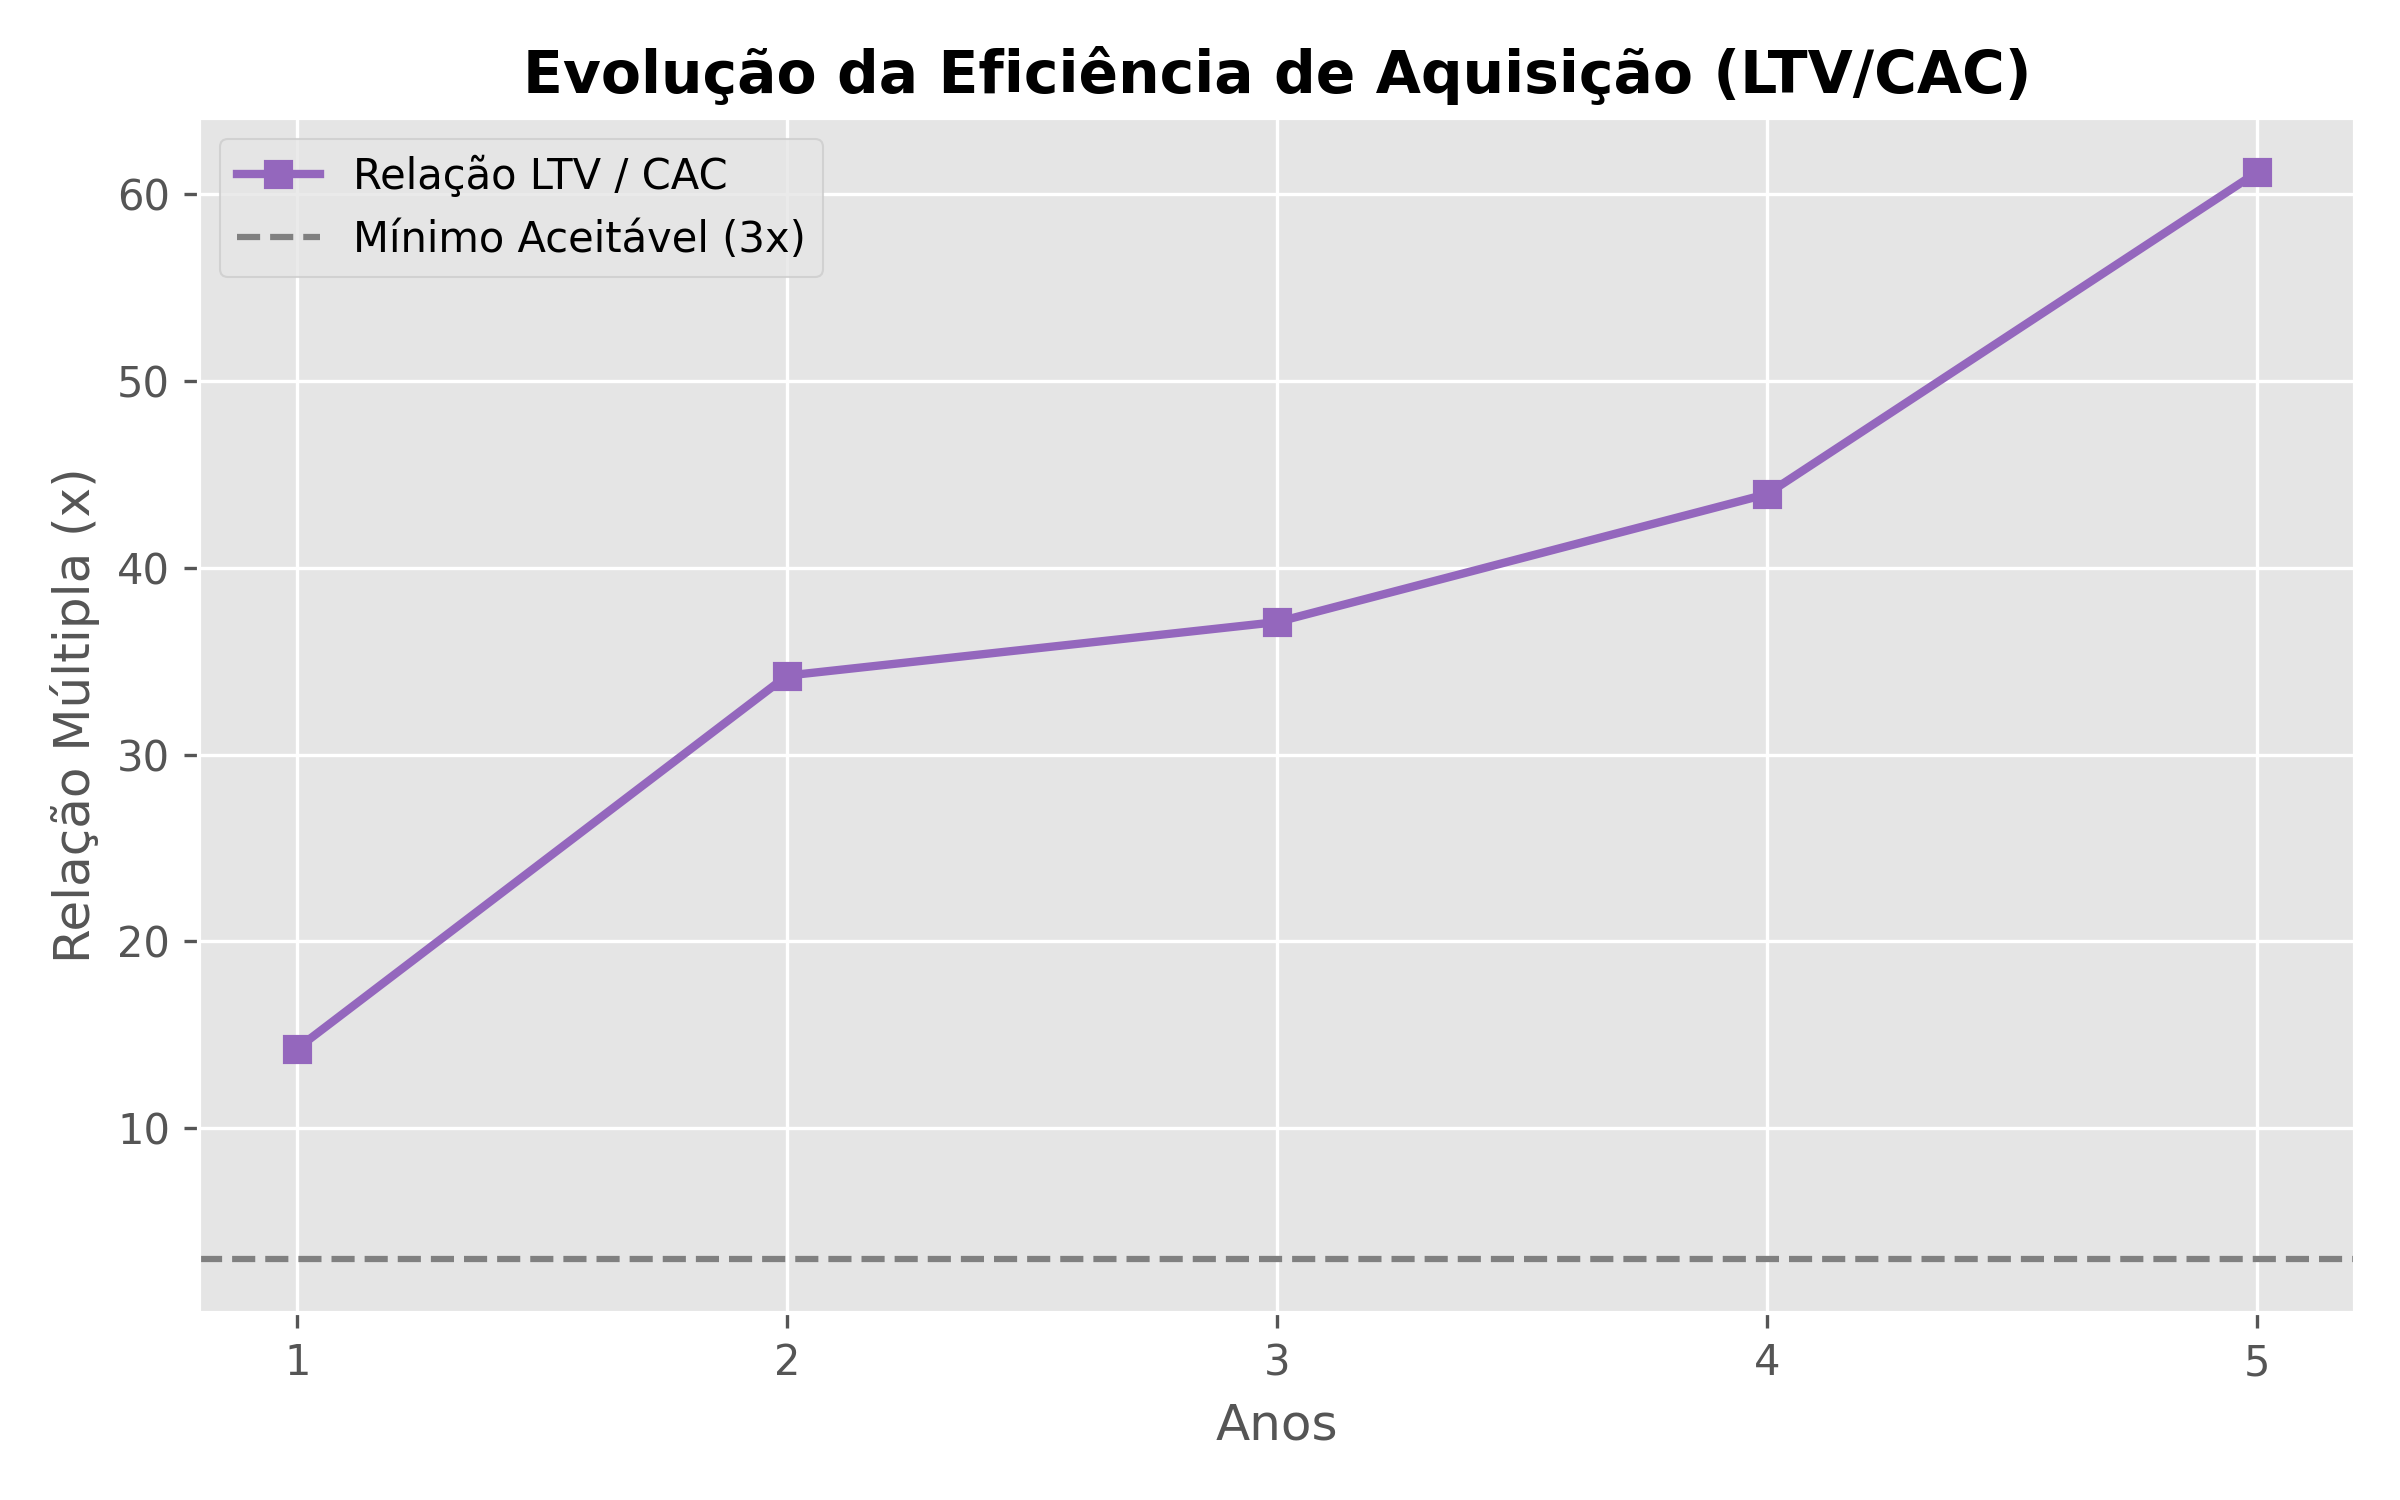
\includegraphics[width=0.85\textwidth]{figuras/grafico_unit_economics.png}
    \caption{Eficiência de Aquisição Conservadora (LTV vs CAC)}
\end{figure}

\subsection{Alocação Orçamentária e Restrição do \textit{Solver}}
Para auditar a coerência do orçamento alocado, utilizamos o algoritmo \textit{Simplex}. O objetivo foi alocar o orçamento de marketing nos canais que, apesar do CAC elevado, conseguissem cobrir a meta comercial.

\begin{figure}[H]
    \centering
    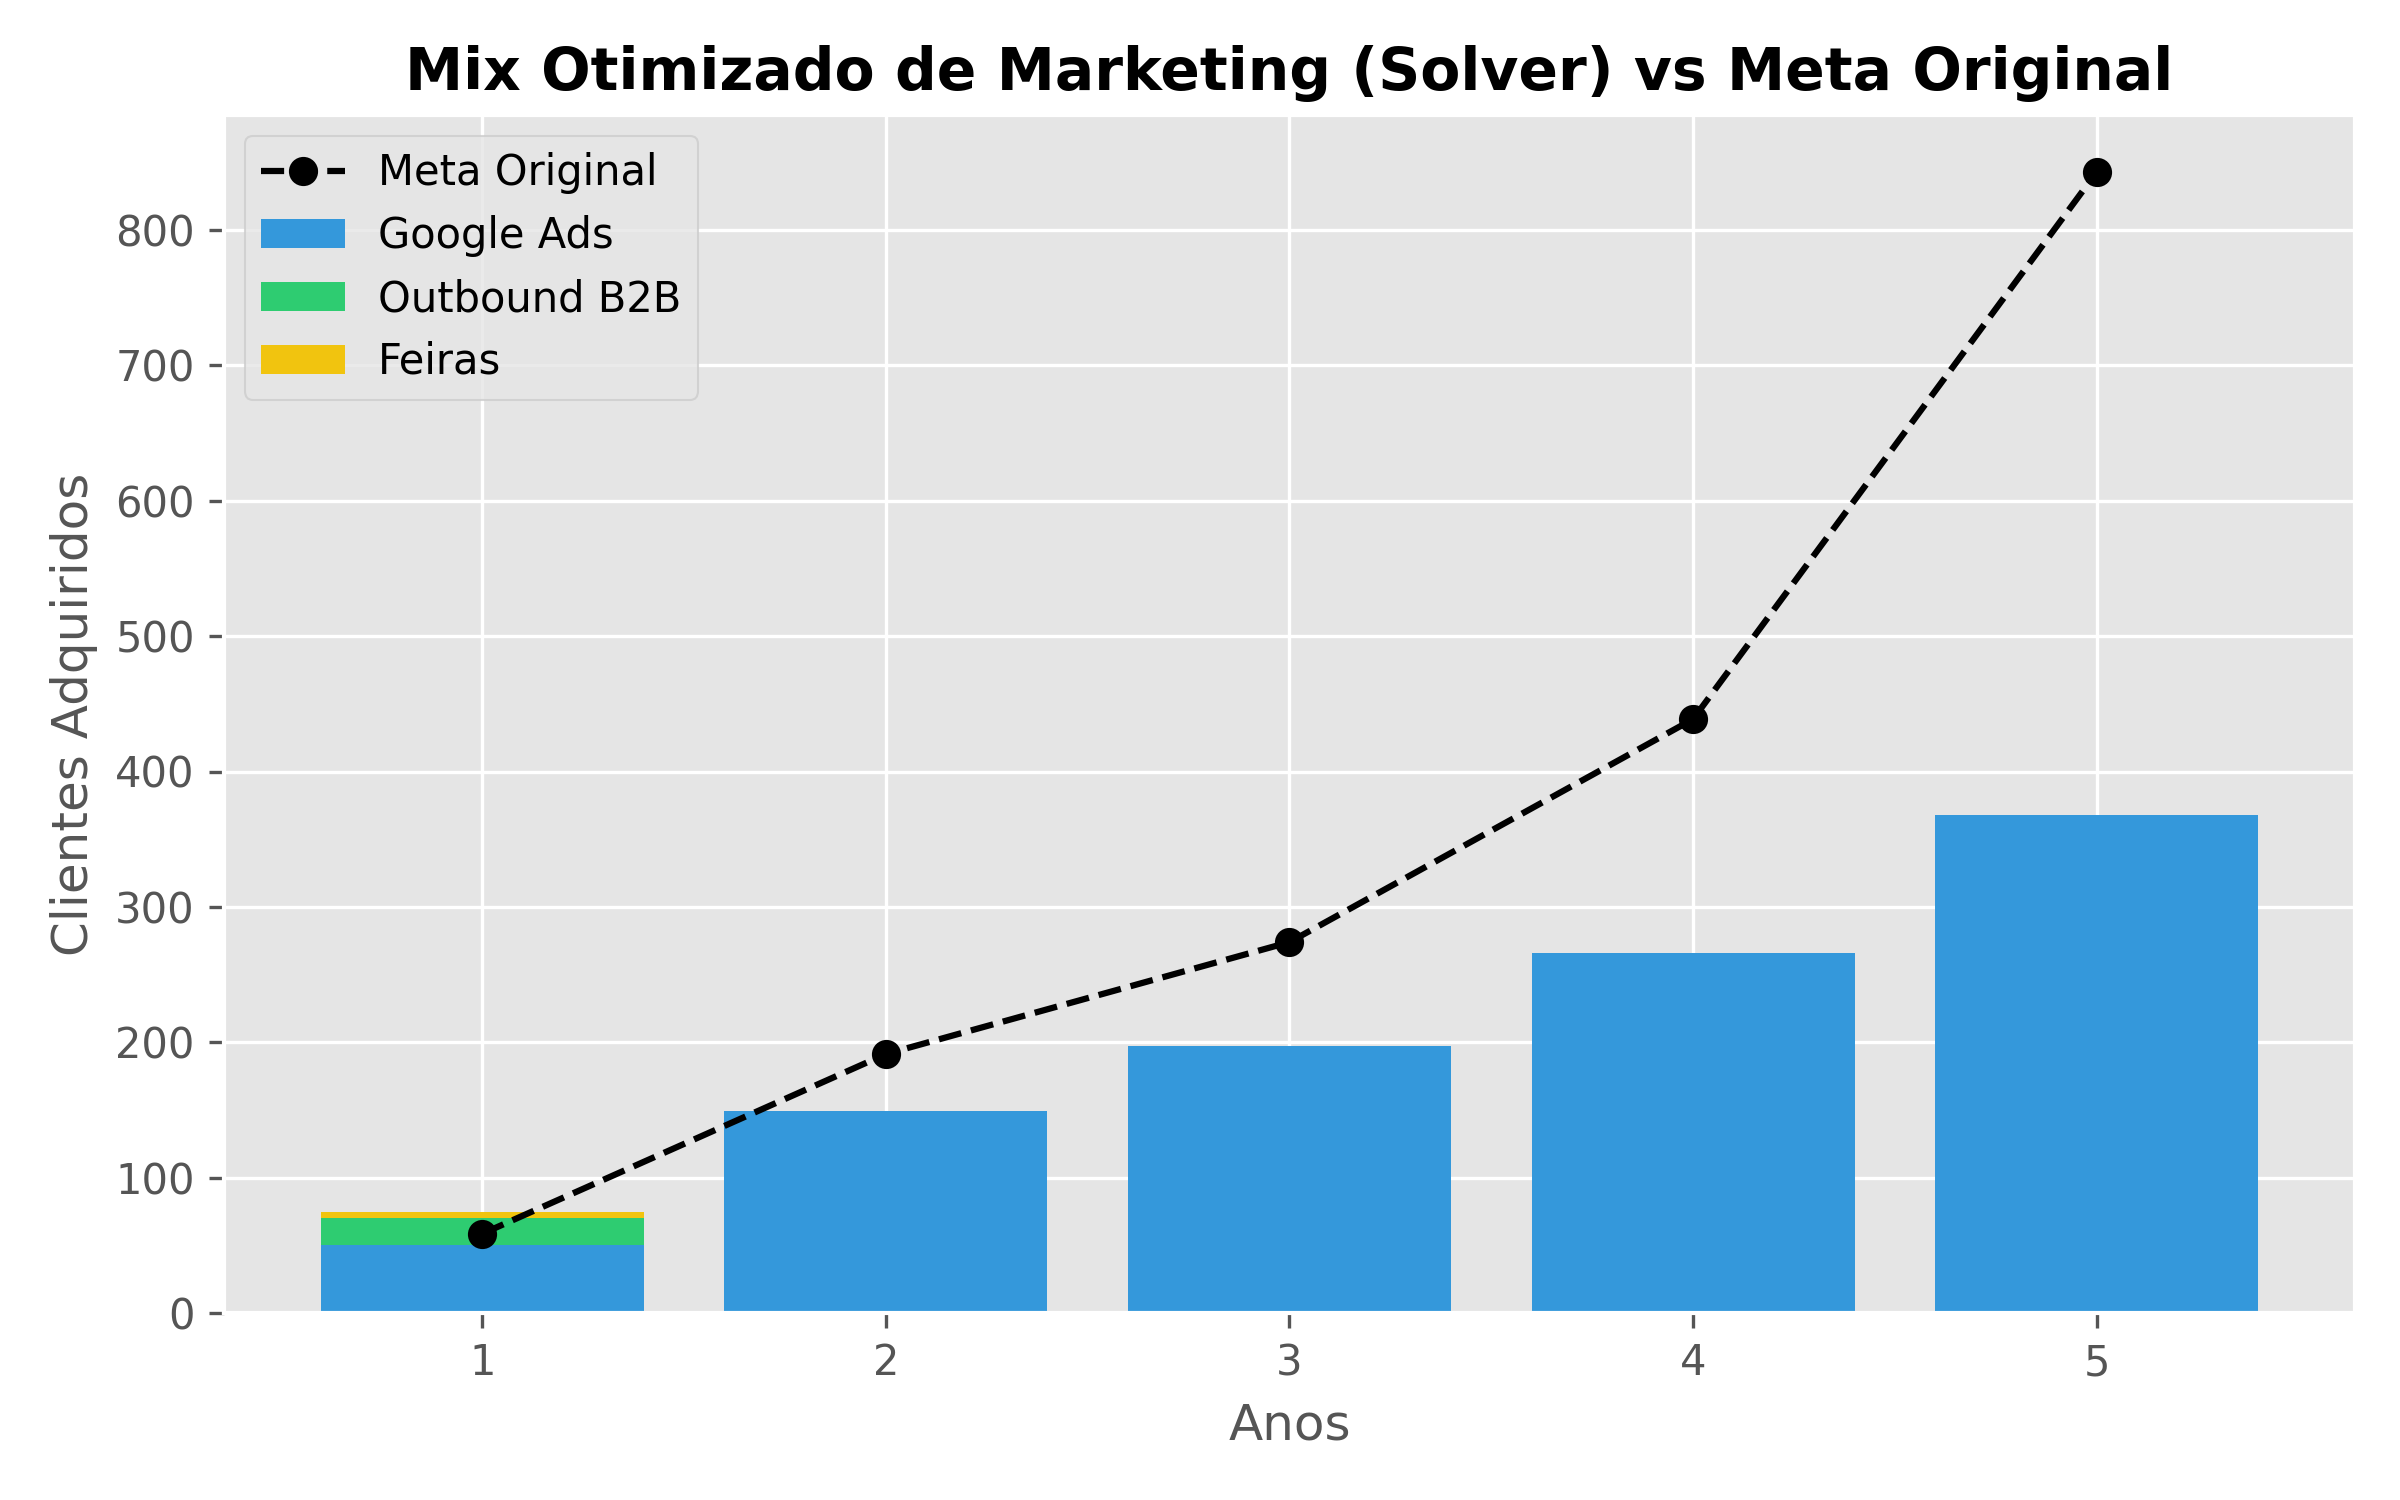
\includegraphics[width=0.85\textwidth]{figuras/grafico_solver_mix.png}
    \caption{Validação de Capacidade Orçamentária via Programação Linear}
\end{figure}

Como observado, a meta é atendida (e superada) até o Ano 3, mas a partir do Ano 4, o *Solver* acusa o esgotamento da verba de aquisição perante o CAC inflado pelas premissas estressadas, sugerindo a necessidade de rodadas de captação subsequentes (Série A/B) para sustentar a máquina comercial.

\section{Dinâmica de Caixa e WACC}
A avaliação de risco reflete a altíssima mortalidade empresarial do setor tecnológico (*early stage*). Para o cálculo do \textit{Weighted Average Cost of Capital} (WACC), incorporamos, sobre o ERP e a Taxa Livre de Risco, um **Prêmio de Startup de 22%**.

Consequentemente, todos os fluxos foram descontados sob um custo de capital extremamente punitivo de \textbf{45,49\% ao ano}.

\begin{figure}[H]
    \centering
    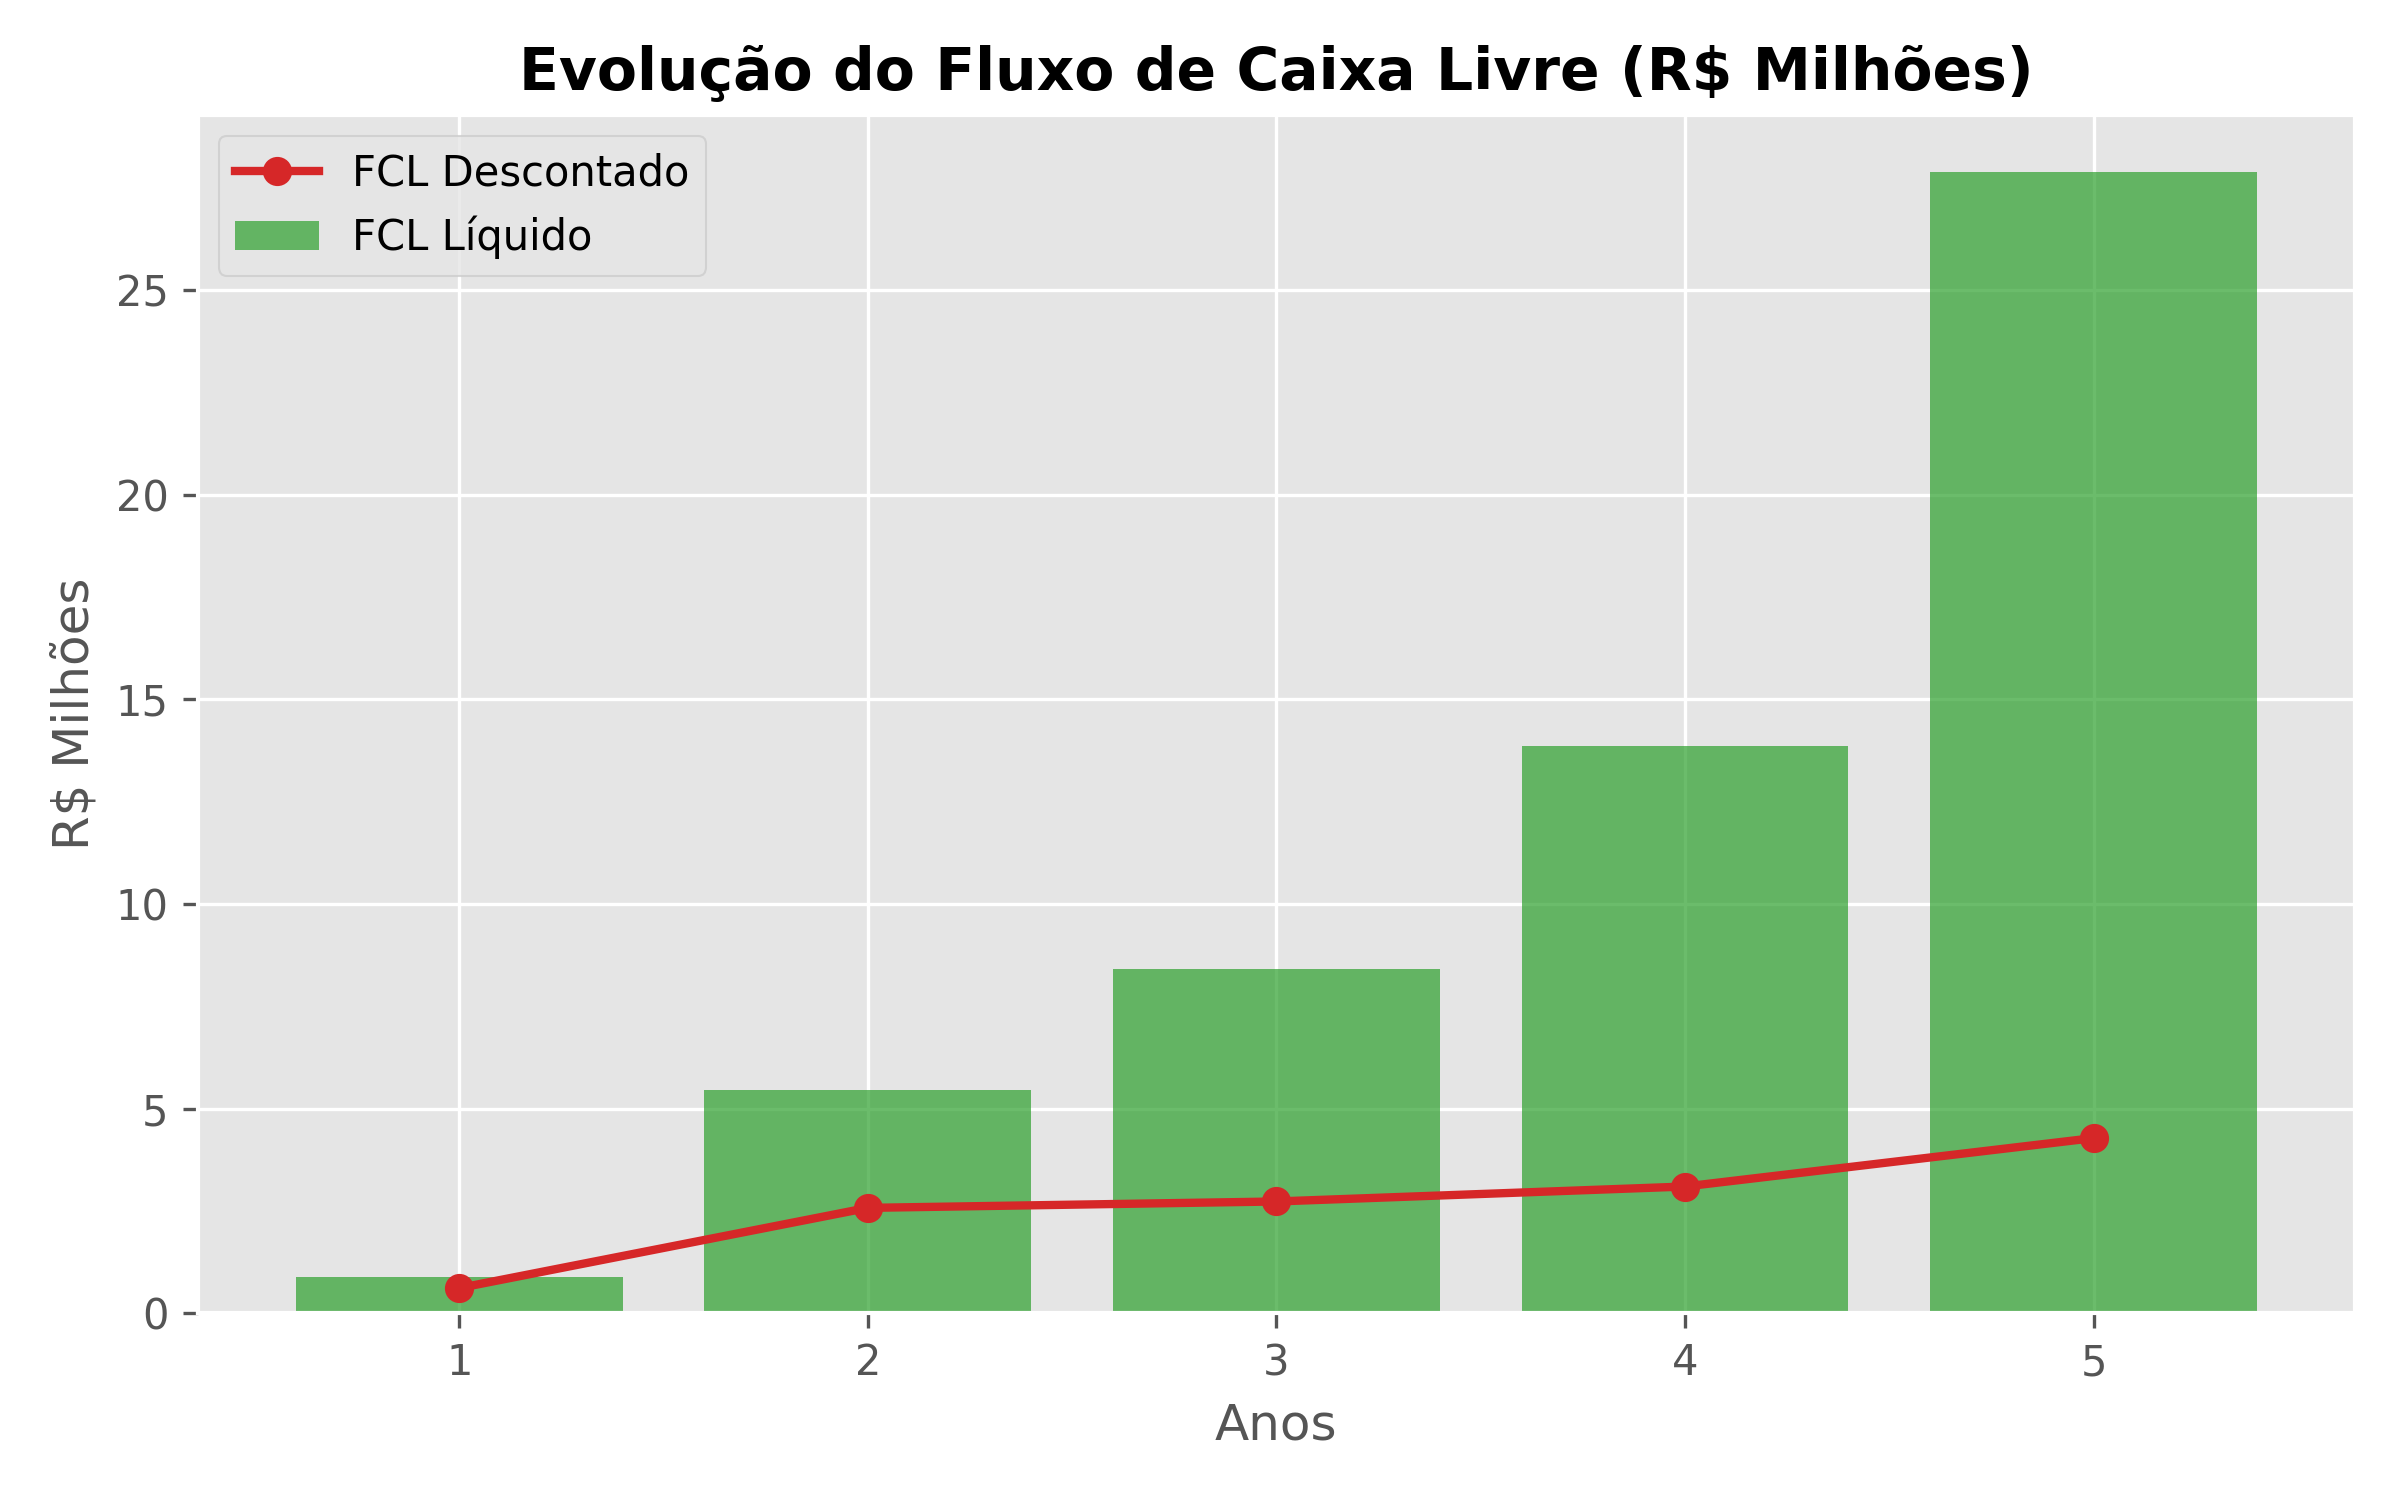
\includegraphics[width=0.85\textwidth]{figuras/grafico_fcl.png}
    \caption{Fluxo de Caixa Livre Descontado a 45,49\% ao ano}
\end{figure}

O fluxo mostra resiliência mesmo frente a taxas predatórias:
\begin{itemize}
    \item \textbf{Investimento Inicial (Fase do Vale da Morte):} R\$ 705.287, refletindo 6 meses de inoperância comercial e o desenvolvimento inicial.
    \item \textbf{VPL Base:} O projeto atinge valor de \textbf{R\$ 12,59 Milhões}.
    \item \textbf{Payback Descontado:} Mesmo sob 45% a.a., o retorno de liquidez ocorre no final do Ano 1.
\end{itemize}

\section{Modelagem Estocástica de Risco (Monte Carlo)}

O determinismo financeiro é incapaz de prever o futuro. Por isso, geramos 2.000 iterações em ambiente computacional variando, simultaneamente:
1. \textbf{WACC:} de 10% a 70\% a.a.
2. \textbf{Taxa de Conversão:} flutuando entre 2% a 8% (cenário pessimista contínuo de *cold call*).

\begin{figure}[H]
    \centering
    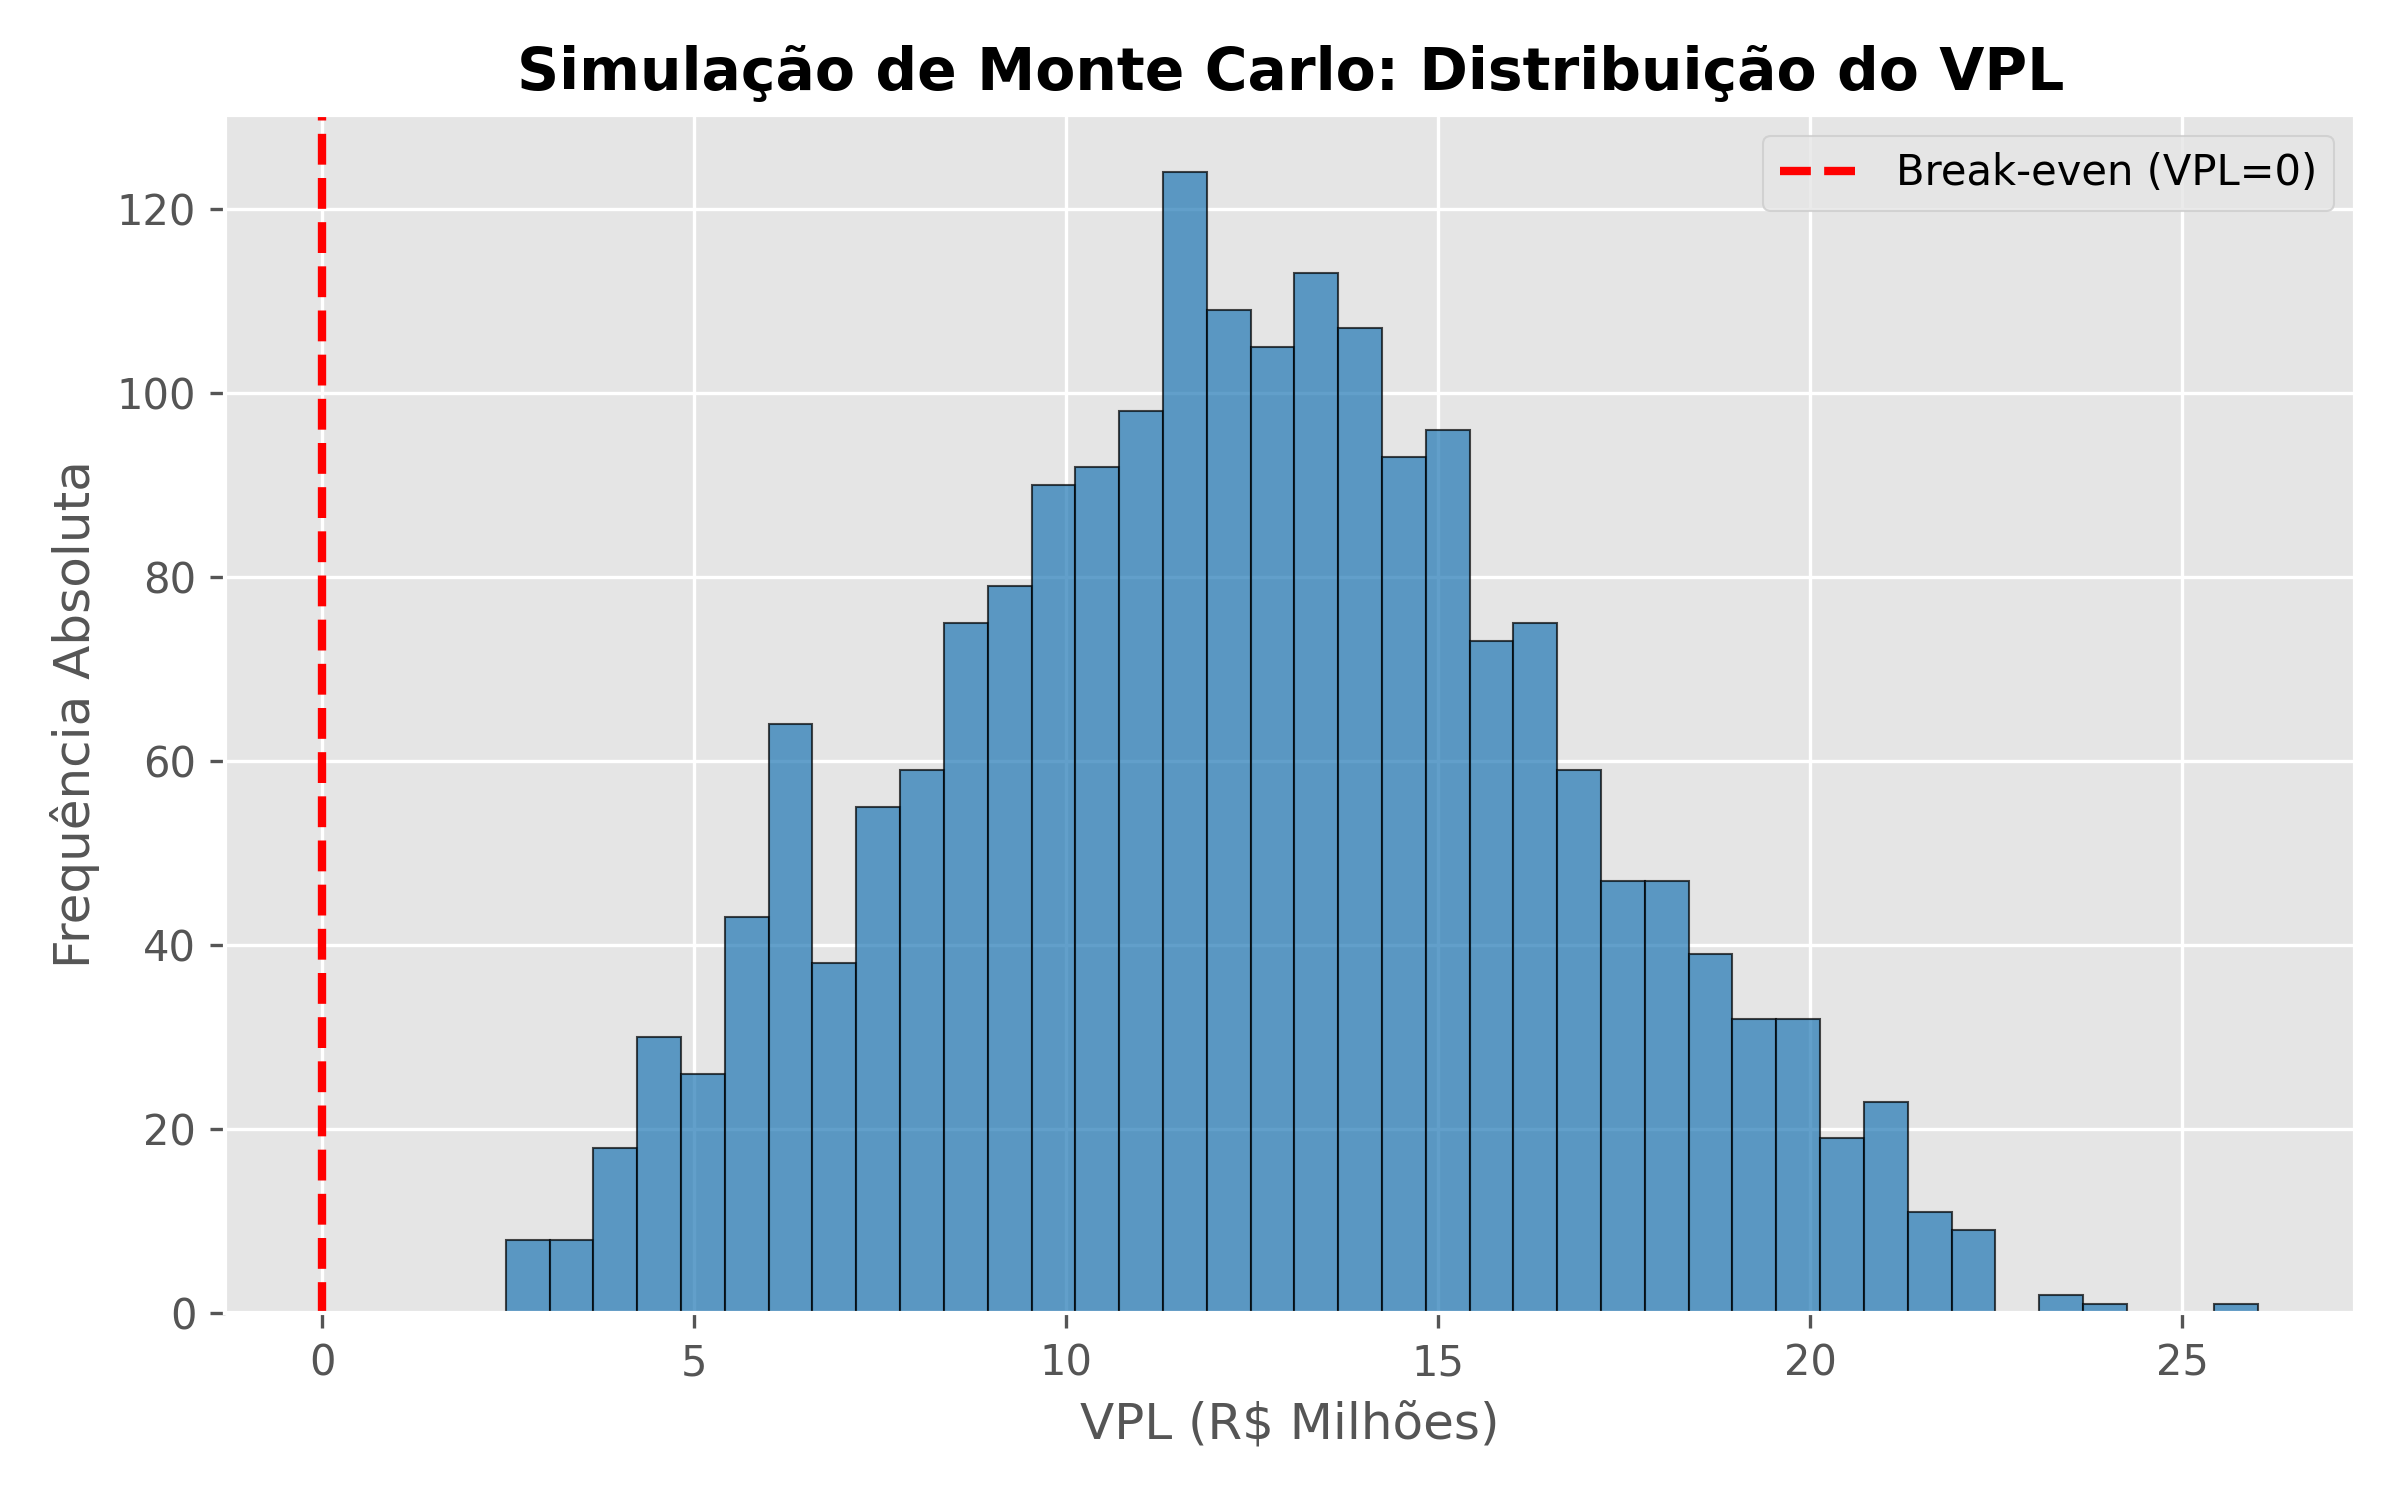
\includegraphics[width=0.85\textwidth]{figuras/grafico_monte_carlo.png}
    \caption{Distribuição de Probabilidades do VPL}
\end{figure}

Ainda que com premissas fortemente desidratadas pelo viés conservador, o modelo sustenta que não há um cenário material em que a startup drene capital indefinidamente sem retorno. O VPL Médio esperado estabilizou em R\$ 12,41 Milhões.

\section{Opções Reais (Valor Estratégico e Ausência de Valor Residual)}

O modelo de opções reais \cite{cox1979} foi aplicado reconhecendo que um *equity* fracassado de tecnologia carece de liquidez.
\begin{enumerate}
    \item \textbf{Opção de Abandono (Put):} Considerando o *feedback* institucional, admitiu-se que o código fonte de uma plataforma sem tração ou clientes não possui valor residual no mercado de M\&A (*Acqui-hire*). Logo, o resgate foi estipulado em R\$ 0,00. A opção tem valor matemático \textbf{nulo}.
    \item \textbf{Opção de Expansão (Call):} Caso o modelo opere no limite superior da simulação de Monte Carlo, os sócios podem exercer a expansão geográfica aportando R\$ 2,5 Milhões no Ano 2. Essa oportunidade (protegida pela assimetria do risco) adiciona \textbf{R\$ 4,43 Milhões} ao *Valuation*.
\end{enumerate}
O VPL Estratégico consolidado é, portanto, de \textbf{R\$ 17,02 Milhões}.

\section{Conclusão}
O modelo apresentado foi purgado de otimismo prematuro. Incorporaram-se a desintermediação de 50\% da receita base, a queima de margem em arranjos de pagamentos (Gateways), e o estrangulamento da máquina de vendas por baixas taxas de conversão (5%). 

Apesar de a métrica de LTV/CAC ser penalizada no limite temporal da Série B devido ao custo inflacionário dos canais tradicionais, a altíssima margem do ticket B2B defende os custos fixos da empresa. O VPL Base final de **R\$ 12,59 Milhões** (descontado sob 45,49\% ao ano) indica de forma sóbria e pragmática que os fundamentos do negócio apresentam resiliência e viabilidade institucional para captações estruturadas do mercado privado (*Venture Capital*).

\newpage
\bibliographystyle{plain}
\bibliography{referencias}

\end{document}
